\section{هدف تمرین}
هدف از این تمرین، توصیف رفتاری یک فلیپ‌فلاپ حساس به لبه با تاخیر ۳ واحد زمانی در زبان \lr{Verilog} و سپس اتصال ساختاری ۳ عدد از آن‌ها به یکدیگر جهت ساخت یک شیفت‌رجیستر (\lr{Shift Register}) سه بیتی است. در این گزارش، عملکرد مدار طراحی‌شده بر روی سیگنال‌های ورودی مشخص‌شده در نمودار زمان‌بندی زیر مورد آزمایش و ارزیابی قرار می‌گیرد.

\begin{figure}[H]
    \centering
    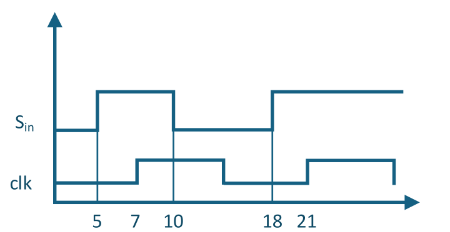
\includegraphics[width=0.6\textwidth]{assets/HW3.png}
    \caption{نمودار زمان‌بندی سیگنال‌های ورودی فرضی تمرین}
\end{figure}

\section{کدهای Verilog}

\subsection{ماژول فلیپ‌فلاپ (\code{dff.v})}
در این بخش، توصیف رفتاری یک فلیپ‌فلاپ \lr{D} حساس به لبه مثبت ساعت آورده شده است که در آن از تاخیر درون‌واگذاری (\lr{intra-assignment delay}) به میزان ۳ واحد زمانی استفاده شده است.

\begin{latin}
    \begin{lstlisting}[language=Verilog]
`timescale 1ns / 1ns
module dff (input clk, input d, output reg q);
    initial begin
        q = 0;
    end

    always @(posedge clk) begin
        q <= #3 d;
    end
endmodule
\end{lstlisting}
\end{latin}

\subsection{ماژول شیفت‌رجیستر (\code{shift\_register\_3bit.v})}
این ماژول با رویکرد ساختاری (\lr{Structural})، سه عدد از فلیپ‌فلاپ‌های تعریف‌شده در مرحله قبل را به صورت زنجیره‌وار به یکدیگر متصل می‌کند تا یک رجیستر انتقال ۳ بیتی شکل بگیرد.

\begin{latin}
    \begin{lstlisting}[language=Verilog]
`timescale 1ns / 1ns
module shift_register_3bit (input clk, input sin, output [2:0] q);
    dff ff0 (clk, sin,  q[0]);
    dff ff1 (clk, q[0], q[1]);
    dff ff2 (clk, q[1], q[2]);
endmodule
\end{lstlisting}
\end{latin}

\subsection{تست‌بنچ (\code{testbench.v})}
ماژول تست‌بنچ وظیفه تولید سیگنال ساعت، اعمال ورودی‌ها دقیقاً مطابق با زمان‌بندی فرضی مسئله و بازنویسی تغییرات سیگنال‌ها در قالب فایل \code{waves.vcd} را بر عهده دارد.

\begin{latin}
    \begin{lstlisting}[language=Verilog]
`timescale 1ns / 1ns
module testbench;
    reg clk;
    reg sin;
    wire [2:0] q;

    shift_register_3bit uut (clk, sin, q);

    always #7 clk = ~clk;

    initial begin
        $dumpfile("waves.vcd");
        $dumpvars(0, testbench);

        $display("Time\t clk\t sin\t q[2:0]");
        $display("-------------------------------");
    end

    always @(clk, sin, q) begin
        #0.1; 
        $display("%2dt\t  %b\t  %b\t  %b", $time, clk, sin, q);
    end

    initial begin
        clk = 0;
        sin = 0;

        #5; sin = 1;
        #5; sin = 0;
        #8; sin = 1;

        #40; $finish;
    end
endmodule
\end{lstlisting}
\end{latin}

\pagebreak

\section{اجرای کد}
برای کامپایل و شبیه‌سازی فایل‌ها در محیط ترمینال لینوکس با استفاده از ابزارهای \lr{iverilog} و \lr{vvp}، دستورات زیر اجرا شده‌اند و خروجی متنی سیستم به شرح زیر است:

\begin{latin}
    \begin{lstlisting}[language=bash]
mohsen@Quanta:/mnt/D/SUT/Term_4/DSD/HW/HW-3$ iverilog -o sim dff.v shift_register_3bit.v testbench.v && vvp sim
VCD info: dumpfile waves.vcd opened for output.
Time     clk     sin     q[2:0]
-------------------------------
 0t       0       0       000
 5t       0       1       000
 7t       1       1       000
10t       1       0       000
10t       1       0       001
14t       0       0       001
18t       0       1       001
21t       1       1       001
24t       1       1       011
28t       0       1       011
35t       1       1       011
38t       1       1       111
42t       0       1       111
49t       1       1       111
56t       0       1       111
testbench.v:38: $finish called at 58 (1ns)
mohsen@Quanta:/mnt/D/SUT/Term_4/DSD/HW/HW-3$ 
\end{lstlisting}
\end{latin}

\section{بررسی سیگنال‌های ورودی و خروجی}
با توجه به نتایج شبیه‌سازی، مشاهده می‌شود که هر لبه مثبت ساعت ورودی \lr{s\_{in}} را نمونه‌برداری می‌کند، اما تغییر خروجی فلیپ‌فلاپ‌ها به دلیل تاخیر ۳ واحد زمانی، دقیقاً ۳ ثانیه (یا واحد زمانی) پس از لبه ساعت اتفاق می‌افتد. این امر باعث می‌شود که داده‌ها گام‌به‌گام و با تاخیر مشخص در طول رجیستر جابه‌جا شوند. شکل موج استخراج‌شده از نرم‌افزار \lr{GTKWave} صحت این رفتار را تایید می‌کند:

\begin{figure}[H]
    \centering
    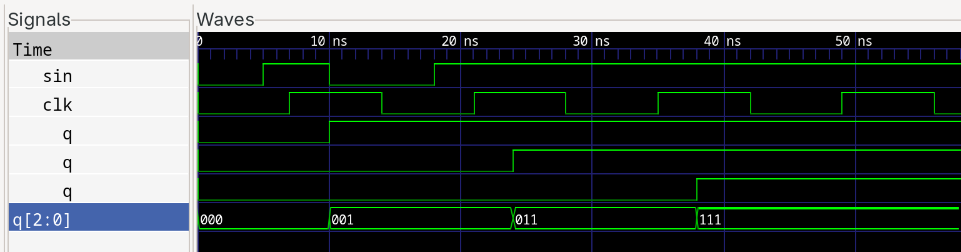
\includegraphics[width=1.0\textwidth]{assets/gtkwave.png}
    \caption{شکل موج سیگنال‌های داخلی و خروجی رجیستر در محیط GTKWave}
\end{figure}